\label{sec:swaption}
To the best of our knowledge, Liu proposed the only implementation of atomic swaption which does not require either blockchain to support smart contracts \cite{liu2018atomic}. Afterward, Tefagh~\etal~ designed atomic bonded cross-chain debt (ABCD) as the first practical cross-chain bond platform in the form of atomic swaptions \cite{tefagh2020atomic}. In this paper, we have designed a more general model of atomic swaption named \emph{\MetaSwaption} which is abstractly shown in Fig~\ref{fig:moc-swaption}.

In what follows, we are going to briefly explain every module of the \MetaSwaption, and through the rest of this paper, we will use this general form as the building block for making some new application-specific swaptions.

\begin{figure}
    \centering
    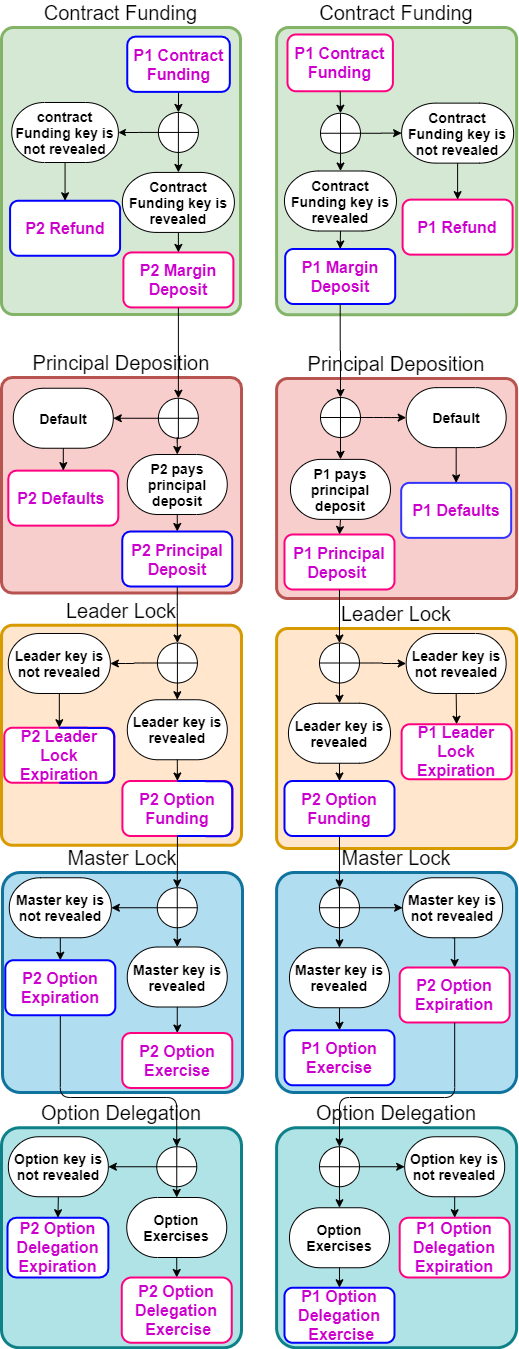
\includegraphics[width=\textwidth,height=\textheight,keepaspectratio]{figures/meta-swaption.png}
    \caption{General overview of the \MetaSwaption}
    \label{fig:moc-swaption}
\end{figure}

Similar to atomic swap and atomic swaption, HTLCs are used so that a party can make decisions by revealing a secret before a locktime or letting the locktime expire. In \MetaSwaption also there are four types of such secrets:
\begin{itemize}
    \item \Aone key
    \item \keyone key
    \item \Atwo key
    \item \Delegation key
\end{itemize}

Note that in HTLC contracts, generaly the locktime of the holder of the secret has to be greater than the other party.
%\ahC{It has to be greater}
% We call the one who buys the swaption, the swpation \SwaptionOwner. In our cases it is mostly Alice.

In the Fig~\ref{fig:moc-swaption}, a \MetaSwaption is 
divided into five different parts, each representing a particular stage in the swaption process. 

Note that in every module introduced in this paper, all transactions in the execution process are exchanged and signed by their corresponding parties before anything goes on chain. During this not-yet-confirmed transactions sharing, all parties are assured that no one can steal their money.


\begin{itemize}

    \item \textbf{Contract funding}: The funding for the swaption buyer (swaption owner) consists of premium and for the seller only margin. Depending on application, the \SwaptionOwner may include margin in her funding.
    The \SwaptionOwner has a relatively small amount of time to reveal \Aone key to buy the option. If she buys the option, premium goes to the seller and margins go to the principal deposition contracts.
    %  Each party sends his margin to a HTLC contract. The swaption buyer also pays a premium to buy the option from the seller. After the exchange of funding transactions, it is time for the swaption buyer to decide weather she buys the option or not. If she reveals the \Aone key, premium goes to the seller and margins go to the margin deposit contracts.
    
    \item \textbf{Principal deposition}: After buying the swpation, each party has to deposit his principal within a specified time interval. If both parties cooperate, the next stage begins.
    The principal deposition transactions might have sighash type of any-one-can-pay\footnote{ANYONECANPAY} since nobody knows all of its inputs in the first place. In this case, since we do not know all the inputs of this transaction at the time of signing, we would not have the correct transaction ID \cite{bip143}. Therefore, we can not create the transactions that get their inputs form this transaction until we discover what all the inputs of the this transaction are going to be. These inputs are only known at the time of broadcasting, not at the time of creating the transactions. So, at the time of creating the transactions in the next stage, the ID of the principal deposition transaction is unknown.
    
    \item \textbf{Leader lock}: Depending on the application, the swaption \SwaptionOwner may decide to use a portion of her option duration as the allowed period of her late principal deposition in order to make money for her principal. In this stage, the party who deposits his principal earlier, \keyone key holder, locks his principal. After assurance of the owner's principal deposition, he is expected to reveal \keyone key determining if the swaption goes to the next stage or not.
    As mentioned in the last stage, the ID of the input of the transactions of this stage is not known at the time of creating. Thus, we have to use the sighash type of no-input\footnote{NOINPUT}\cite{bip118} that allows us to create a transaction where none of its inputs are known. So, by this sighash we can create the transactions in the leader lock stage without any inputs. Later, at the time of broadcast, since the inputs of the principal deposition transaction are known and consequently we have its ID, we can use this transaction as an input for the transactions of the leader lock stage and broadcast them.
    
    \item \textbf{Master lock}: In this stage, the \SwaptionOwner (\Atwo key holder) chooses weather she exercises the option or not using \Atwo key. By exercising the option, principals are exchanged and the swaption ends. By not revealing \Atwo key, letting the locktime expire, next stage begins. Like the last stage, since the inputs of the parent transaction of the transactions of this stage are not clear, we have to use the no-input sighash.
    
    \item \textbf{Option delegation}: This stage might be utilized in certain use-cases such as futures arbitrage discussed later. For fixing the problem of cyclic locktimes in master lock stage, we develop a method to delegate the option from \SwaptionOwner to another desired party. The newly promoted party can later decide the execution of the swaption by the \Delegation key. In this stage, like last two stages we have to use the no-input sighash.

    % \item \textbf{Trust box}: In some cases, i.e. futures arbitrage, the \SwaptionOwner needs to transfer the right of signing some transactions to a party other than swaption buyer or seller. The extents of trust box may differ for each use-cases of \MetaSwaption instances.
    % \ahC{Is this paragraph needed anymore?}
\end{itemize}

When using the no-input sighash, the party signs the transaction without specifying its inputs, so a malicious party has the ability to give any UTXO that belongs to the public key of this party. Hence, each party has to create a separate public key for each transaction that she makes.
Using the stages described above, we can generate new instances of \MetaSwaption targeting swaptions or bonds. Based on different goals, we can choose which of these stages appear in our instance. In the following subsections, we describe different swaptions devised for a variety of use-cases:
\begin{itemize}
    \item Early deposition swaption
    \item Late deposition swaption
    \item Margin-free limited swaption
\end{itemize}
Notice that in Fig~\ref{fig:swaption-early-deposition}, Fig~\ref{fig:swaption-late-deposition}, and Fig~\ref{fig:swaption-margin-free-limited} the locktimes $P$,$T$,$M$,$E$, and $T'$ are calculated with respect to  a common origin of time. In other words, the current time of the swaption establishment has to be added to all the locktimes shown in these stages, because they are not relative but absolute times. 
% Each of these components has different procedure. For further analysing the effectiveness of each component, we design a time elapsed experiment aiming to analyse the worst case running time of them.


% \begin{experiment}
% {Time Elapsed}\\
% Given $p_{buyer}$ and $p_{seller}$ the buyer and the seller of the component $\mathcal{C}$, the $\mathcal{T}[\mathcal{C}]$ is the minimum spend locktime during the execution runtime of $\mathcal{C}$ if $p_{seller}$ adversarially waits in every steps until the last moments.
% \end{experiment}

% We discus the second type in detail. The other types are discussed in \Apn{\ref{app:conv-swaption}} and \Apn{\ref{app:margin-free-swaption}}.

% \ahC{Somewhere we have to mention that we split the option time into two parts, one is time for revealing \keyone key and the other one is \Atwo key. Then we can say that Alice is settling other swaptions in the case of arbitrage during option time.}



\subsection{Early Deposition Swaption}
\label{app:conv-swaption}

This type of swaption is the conventional form that is first introduced in \cite{liu2018atomic}. Alice wants to exchange her ACoins with Bob's BCoins. We rebuild this type with our \MetaSwaption extended form in the way depicted in Fig~\ref{fig:swaption-early-deposition}. We begin analysing each stage of this type by explaining every possible scenarios as follows:

\begin{itemize}
    \item \textbf{Contract funding}: Alice and Bob broadcast their funding transactions. Alice's includes margin and premium and Bob's includes margin worth equal to Alice's margin.
    
    \item \textbf{Principal deposition}: In this stage, Bob is waiting for Alice to deposit her principal. There are two possible scenarios:
    \begin{itemize}
        \item Alice does not deposit her principal. In this case, Bob also defaults and their margins are exchanged.
        \item Alice deposits her principal but Bob does not. In this case, Alice is in master lock stage. So, she reveals \Atwo and takes Bob's margin besides her own principal.
        % Alice is already in option contract stage and she can take the ownership of both her principal and Bob's margin by revealing the \Atwo key and broadcasting Bob's default transaction.
    \end{itemize}
     But if Bob fails to deposit his principal, 
    
    \item \textbf{Master lock}: If both parties go to this stage, Alice can then use her option as mentioned earlier.
\end{itemize}

\begin{figure}
    \centering
    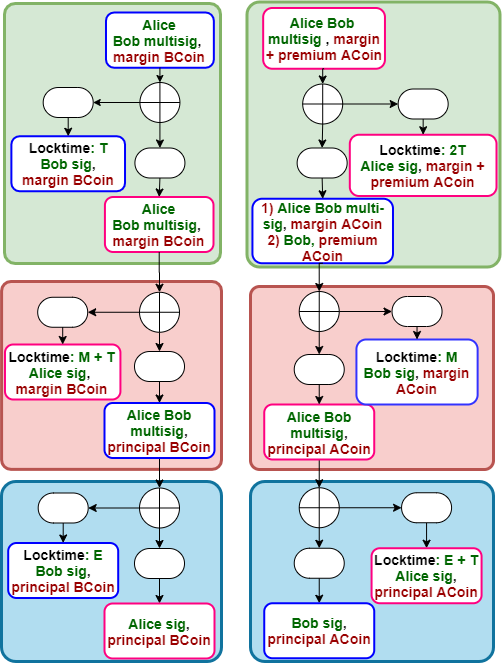
\includegraphics[width=\textwidth]{figures/early dep.png}
    \caption{Early deposition swaption where the buyer (Alice) deposits her principal earlier than the seller (Bob). The pink-bordered transactions are broadcasted by Alice and the blue-bordered ones by Bob.}
    \label{fig:swaption-early-deposition}
\end{figure}
% \ahC{Shall we mention that 546 Satoshis can not be counted as margin?}


\subsection{Late Deposition Swaption}
In this type of swaption the swaption \SwaptionOwner, Alice, needs the seller, Bob, to deposit his principal before her, so that she can settle other deals on other contracts before depositing her principal in this swaption. Alice can exploit this type of swaption in the situations where she does not own enough budget for her principal and she is going to make the required amount of capital using what she has takes from Bob. Since Bob has to wait a longer time for Alice to deposit, Alice has to pay more amount of premium compared to the early deposition swaption.
One example use-case can be the futures arbitrages which will be discussed later. The overview of this swaption is shown on Fig.~\ref{fig:swaption-late-deposition}.

\begin{itemize}
    \item \textbf{Contract funding:} The two parties broadcast their funding transactions. Alice includes margin in her funding and an amount of guarantee is added to Bob's funding besides his margin. We can use this guarantee amount to punish Bob in case of cheating. If he behaves normally, the guarantee will return back to him. The amount of guarantee is negotiable depending on the use-case.
    
    \item \textbf{Principal deposition:} When this stage begins Alice is waiting for Bob to deposit his principal. If Bob defaults, then Alice has two options to punish him:
    \begin{itemize}
        \item She defaults, loses her margin and takes Bob's guarantee and margin.
        \item She deposits her principal and enters the next stage.
    \end{itemize}

    \item \textbf{Leader lock}: 
    There are four possible scenarios:
    \begin{itemize}
        \item In the last stage, Bob deposited his principal but Alice did not. Now Bob does not reveal \keyone key, so that Alice's margin is exchanged with Bob's margin.
        \item Both have deposited their principals and Bob does not reveal \keyone key. Broadcasting the Alice's leader lock transactions, Alice gets Bob's guarantee.
        \item In the last stage, Alice deposited her principal but Bob did not (Second way to punish Bob). Now Alice broadcasts the Alice's leader lock expiration transaction and takes all of her principal back in addition to Bob's margin and guarantee that she has previously taken in the last stage. 
        \item Both have deposited their principals. Bob reveals \keyone key and take back his guarantee. Afterward, they go to the next stage.
    \end{itemize}
    
    \item \textbf{Master lock}: It is the time for Alice to use her option. She either exercises and principals are exchanged or reveals nothing and each party gets his principal back.
\end{itemize}


\begin{figure}
    \centering
    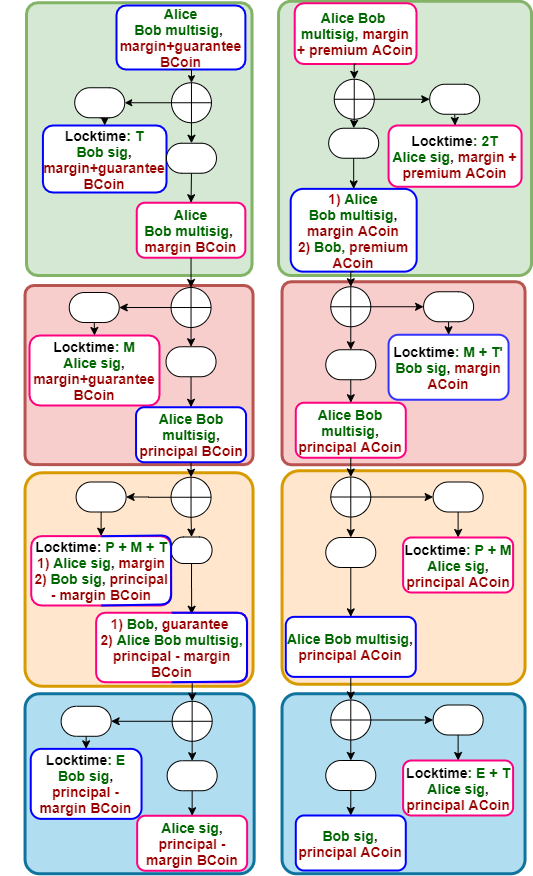
\includegraphics[width=\textwidth,height=0.93\textheight,keepaspectratio]{figures/late dep.png}
    \caption{Late deposition swaption where the seller (Bob) deposits his principal earlier than the buyer (Alice). Pink-bordered transactions are broadcast by Alice and blue-bordered ones by Bob.}
    \label{fig:swaption-late-deposition}
\end{figure}

% Note that since Bob's only incentive is the premium (and not the margin), it is not possible that Alice uses this swaption alongside with other swaptions. For instance, in the case that Alice uses Bob's principal as her principal in another swaption, Bob can cheat on Alice by pretending to be a different person and act as the other party in the second swaption as well as the first one. Then he can steal Alice's premium in the second swaption by not exposing the \keyone key. 
% Later we will prove that Alice can only use one premium guarantee in a set of swaptions which are expected to be exercised in one run simultaneously. Because every run must have only one \keyone and \Atwo and \Aone key which is impossible when we use multiple premium guarantee boxes.
% It is not possible to allow Alice to send the premium of other swaption in directly with usage of another Premium Guarantee 
%\ahC{This section is changed and it is no longer standalone. Still move to appendix?}
% The detailed process of this swaption is written in \Apn{\ref{app:margin-free-swaption}} 
% \ref{app:margin-free-swaption}.



% \subsection{Atomic Non-collateralized Loan}
% A modification of the {\it Late-Deposition swaption} in which Alice does not have to deposit any margin before she gets Bob's principal has the functionality of a loan with no collateral needed. As mentioned in \cite{liu2018atomic} it is not possible to have no margin for the buyer if the parties are on different blockchains. \fatemeC{explain more} Hence, in order to have this loan, the parties have to be on the same chain. 



\subsection{Margin-Free Limited Swaption}

\label{app:margin-free-swaption}
Until now, it was believed that Alice's margin deposit is necessary due to the limitations of HTLCs \cite{liu2018atomic}. In this work, we propose a novel approach which allows Alice to participate in a swaption without depositing any margin.
In the beginning of contract, Bob deposits an amount of BCoin as guarantee which is sent to Alice directly by revealing \Aone key. Alice also adds an amount of ACoin equal to Bob's guarantee to her premium, though none of them will be directly sent to Bob. Later, the premium and guarantee go to Bob in all possible situations except where Bob refuses to reveal the \keyone key when Alice does not default, then he will be punished by not getting back his guarantee.
% In Fig~ \ref{fig:swaption-margin-free-limited} we use our getting a guarantee money from Bob to build the {\it Margin Free} swaption.
% In this type besides premium, Alice deposits an amount of ACoiun equal to Bob's guarantee. Her premium is not paid directly after revealing of \Aone key, but instead will be locked until Bob acts honestly up to end of the Leader Lock stage.
% Later the premium goes to Bob in all possible situations except where Bob refuses to reveal the \keyone key and he will be punished by not paying back his guarantee. 
The amount of guarantee can vary depending on the Alice's need. In next section, we will explain the limitation imposed on the amount of guarantee in details. The execution procedure of the margin-free swaption is as follows:
\begin{itemize}
    \item \textbf{Contract funding}: Bob pays his margin plus an amount of guarantee which prevents him from cheating in later stages. Alice also pays extra premium which in the case of Bob's honest behaviour pays back the guarantee to Bob. Guarantee in the Bob's section is directly sent to Alice after revealing the \Aone key. 
    
    \item \textbf{Principal deposition}: This stage is the same as previous principal deposition stages for Bob. He has M locktime to deposit his principal. If he does not, Alice takes his margin. In Alice's section, either she defaults and gives Bob the premium or she deposits her principal and goes to the next stage waiting for Bob to reveal the \keyone key.
    % \item \textbf{Premium Guarantee}: Either Alice defaults and gives Bob the premium or she deposits her principal and goes to the next stage waiting for Bob to reveal the \keyone key.
    
    \item \textbf{Leader key}: If Bob has not deposited his principal until M locktime, Alice will also avoid depositing her principal and gives Bob the premium and ACoin guarantee while getting his margin from him.
    % and Alice has two options ahead: 1)She deposits her principal before M + T, then broadcasts the \keyone key expiration transaction, in which her premium is refunded. Therefore, if Bob defaults and Alice does not, there would be no premium for Bob. In any other situation he gets the premium. 
    If both parties have deposited their principals when this stage begins, Bob's decision whether to reveal the \keyone key or not, determines the future of the swaption. If he refuses to reveal, he takes his own money back and Alice takes her own money including premium back. In this case, Bob loses his guarantee as a punishment. Otherwise, if he reveals the \keyone key, they both go to the next stage waiting for Alice to exercise her option. Additionally, by revealing the \keyone key, Bob finishes his task and it is the time to send back his guarantee. Hence at the end of this stage, Bob's guarantee will be paid back to himself.
    
    \item \textbf{Option funding}: This stage is similar to the last versions of swpation.
\end{itemize}

\begin{figure}
    \centering
    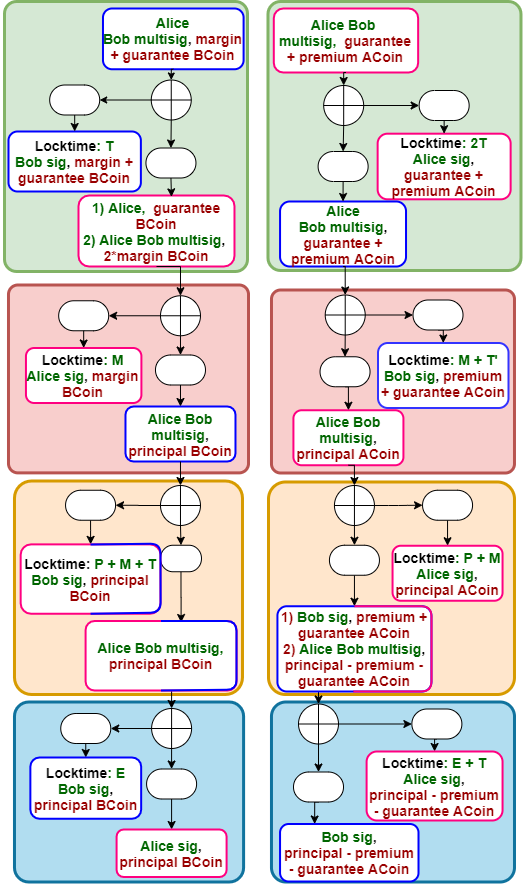
\includegraphics[width=\textwidth,height=0.93\textheight]{figures/swaption-margin-free.png}
    \caption{Margin-free limited swpation where the buyer (Alice) is not supposed to deposit any margin. Pink-bordered transactions are broadcasted by Alice and blue-bordered ones by Bob.}
    \label{fig:swaption-margin-free-limited}
\end{figure}
% \fatemeC{mention auction as an application for the margin-free swaption. you can use the aucion section primarily written}

Locktimes in all of these swaptions have to stick to some general rules: 
\begin{itemize}
    \item $T$ is the minimum amount of time or number of blocks needed for a mined transaction to be confirmed. In bitcoin it is $6$ blocks which is approximately achieved in 1 hour.
    
    \item $M$ is the time for Bob to deposit principal. Hence, can be equal or greater than $T$.
    
    \item $T'$ can be relatively large, since it gives Alice the time she needs to deposit her principal.
    
    \item $P$ is the locktime that Bob has to reveal the \keyone key. This has to be larger than $T'$ so that Alice has to deposit before Bob's revealing time elapses.
    
    \item $E$ is the time for Alice's option exercise which can be relatively large, since it is an option.
\end{itemize}
Note that we use $T$ to make two locktimes differ in a reasonable amount of time to prevent cheating. However, this is the minimum difference needed. Hence, everywhere $T$ is used, we can replace it with different larger values. We use $T$ for simplicity though.